\documentclass[tikz,border=5mm]{standalone}
\usepackage[T1]{fontenc}
\usepackage{circuitikz}
\usepackage{amsmath}
\usetikzlibrary{arrows.meta,backgrounds,calc}

% Coil, magnetic core and normally-open contact, matching the supplied symbol.
\tikzset{pics/reed relay/.style={code={
  \draw[line width=0.8pt] (-0.95,-0.7) -- (-0.95,-0.55);
  \foreach \turn in {0,...,4} {
    \pgfmathsetmacro{\ya}{-0.55+0.22*\turn}
    \pgfmathsetmacro{\yb}{\ya+0.22}
    \draw[line width=0.8pt] (-0.95,\ya)
      .. controls (-0.57,\ya) and (-0.57,\yb) .. (-0.95,\yb);
  }
  \draw[line width=0.8pt] (-0.95,0.55) -- (-0.95,0.7);
  \draw[line width=1.2pt] (-0.43,-0.55) -- (-0.43,0.55);
  \draw[line width=0.8pt] (0,0.7) -- (0,0.27);
  \draw[line width=0.8pt] (0,-0.7) -- (0,-0.27);
  \draw[line width=0.8pt] (0,0.21) circle[radius=0.06];
  \draw[line width=0.8pt] (0,-0.21) circle[radius=0.06];
  \draw[line width=0.8pt] (0.04,-0.16) -- (0.27,0.18);
}}}

% ---------------------------------------------------------------------------
% Anti-series (push-pull) balanced APD pair, shared TIA, single-rail autobalance.
%
% Diode orientation: both pD are drawn bottom-to-top, so each has its ANODE at
% the lower coordinate and its CATHODE at the upper one:
%     D+ : cathode -> V_B+          , anode   -> summing node
%     D- : cathode -> summing node  , anode   -> V_B-
% Both are reverse biased; photocurrent runs DOWNWARD through the stack.
% The TIA holds the midpoint at virtual ground and absorbs only (i+ - i-).
%
% C_b: provisional 100 nF effective capacitance per bias rail to analog ground.
%   Local bypass at the diode bias terminal, not across the TIA input.
%   Ideal |Z_C| = 1/(2 pi f C_b): 1.59 ohm at 1 MHz, 0.159 ohm at 10 MHz.
%   No series bias resistor: no standalone RC filter or resistive current limit.
%   Actual impedance includes regulator output impedance, ESR, ESL and layout.
%   Voltage rating, bias derating, regulator stability and fault current need
%   validation with the actual positive/negative bias supplies.
%
% Autobalance: V_out itself is the differential DC error variable. A follower
%   isolates the TIA from a 1 kHz RC low-pass and its contact network. A PI
%   controller command is V_ref, applied to the post regulator reference input.
%   U_trim is a series voltage drop between the fixed V_B+ rail and upper bias node.
%   It has no ground connection; the upper bias is V_B+ - U_trim.
%   LPF stays connected in every mode. U3A selects PI/fixed reference;
%   U3B resets the PI in states 0--2. No K_AB or separate LPF clamp.
%   Both SPDT symbols depict mode 3: U3A selects A, U3B selects B.
%   A command RC filter after S_ref is on this board, before the regulator
%   interface. Its nominal model includes 120 ohm switch on-resistance at
%   +/-15 V, with a high-Z load and negligible selected-source impedance.
%   Switching sequence and plant stability still require validation.
%
% K+/K- are normally-open reed contacts; their coils are electrically isolated
% from the photodiode path. The bar beside each coil is the magnetic core.
% ---------------------------------------------------------------------------

\begin{document}
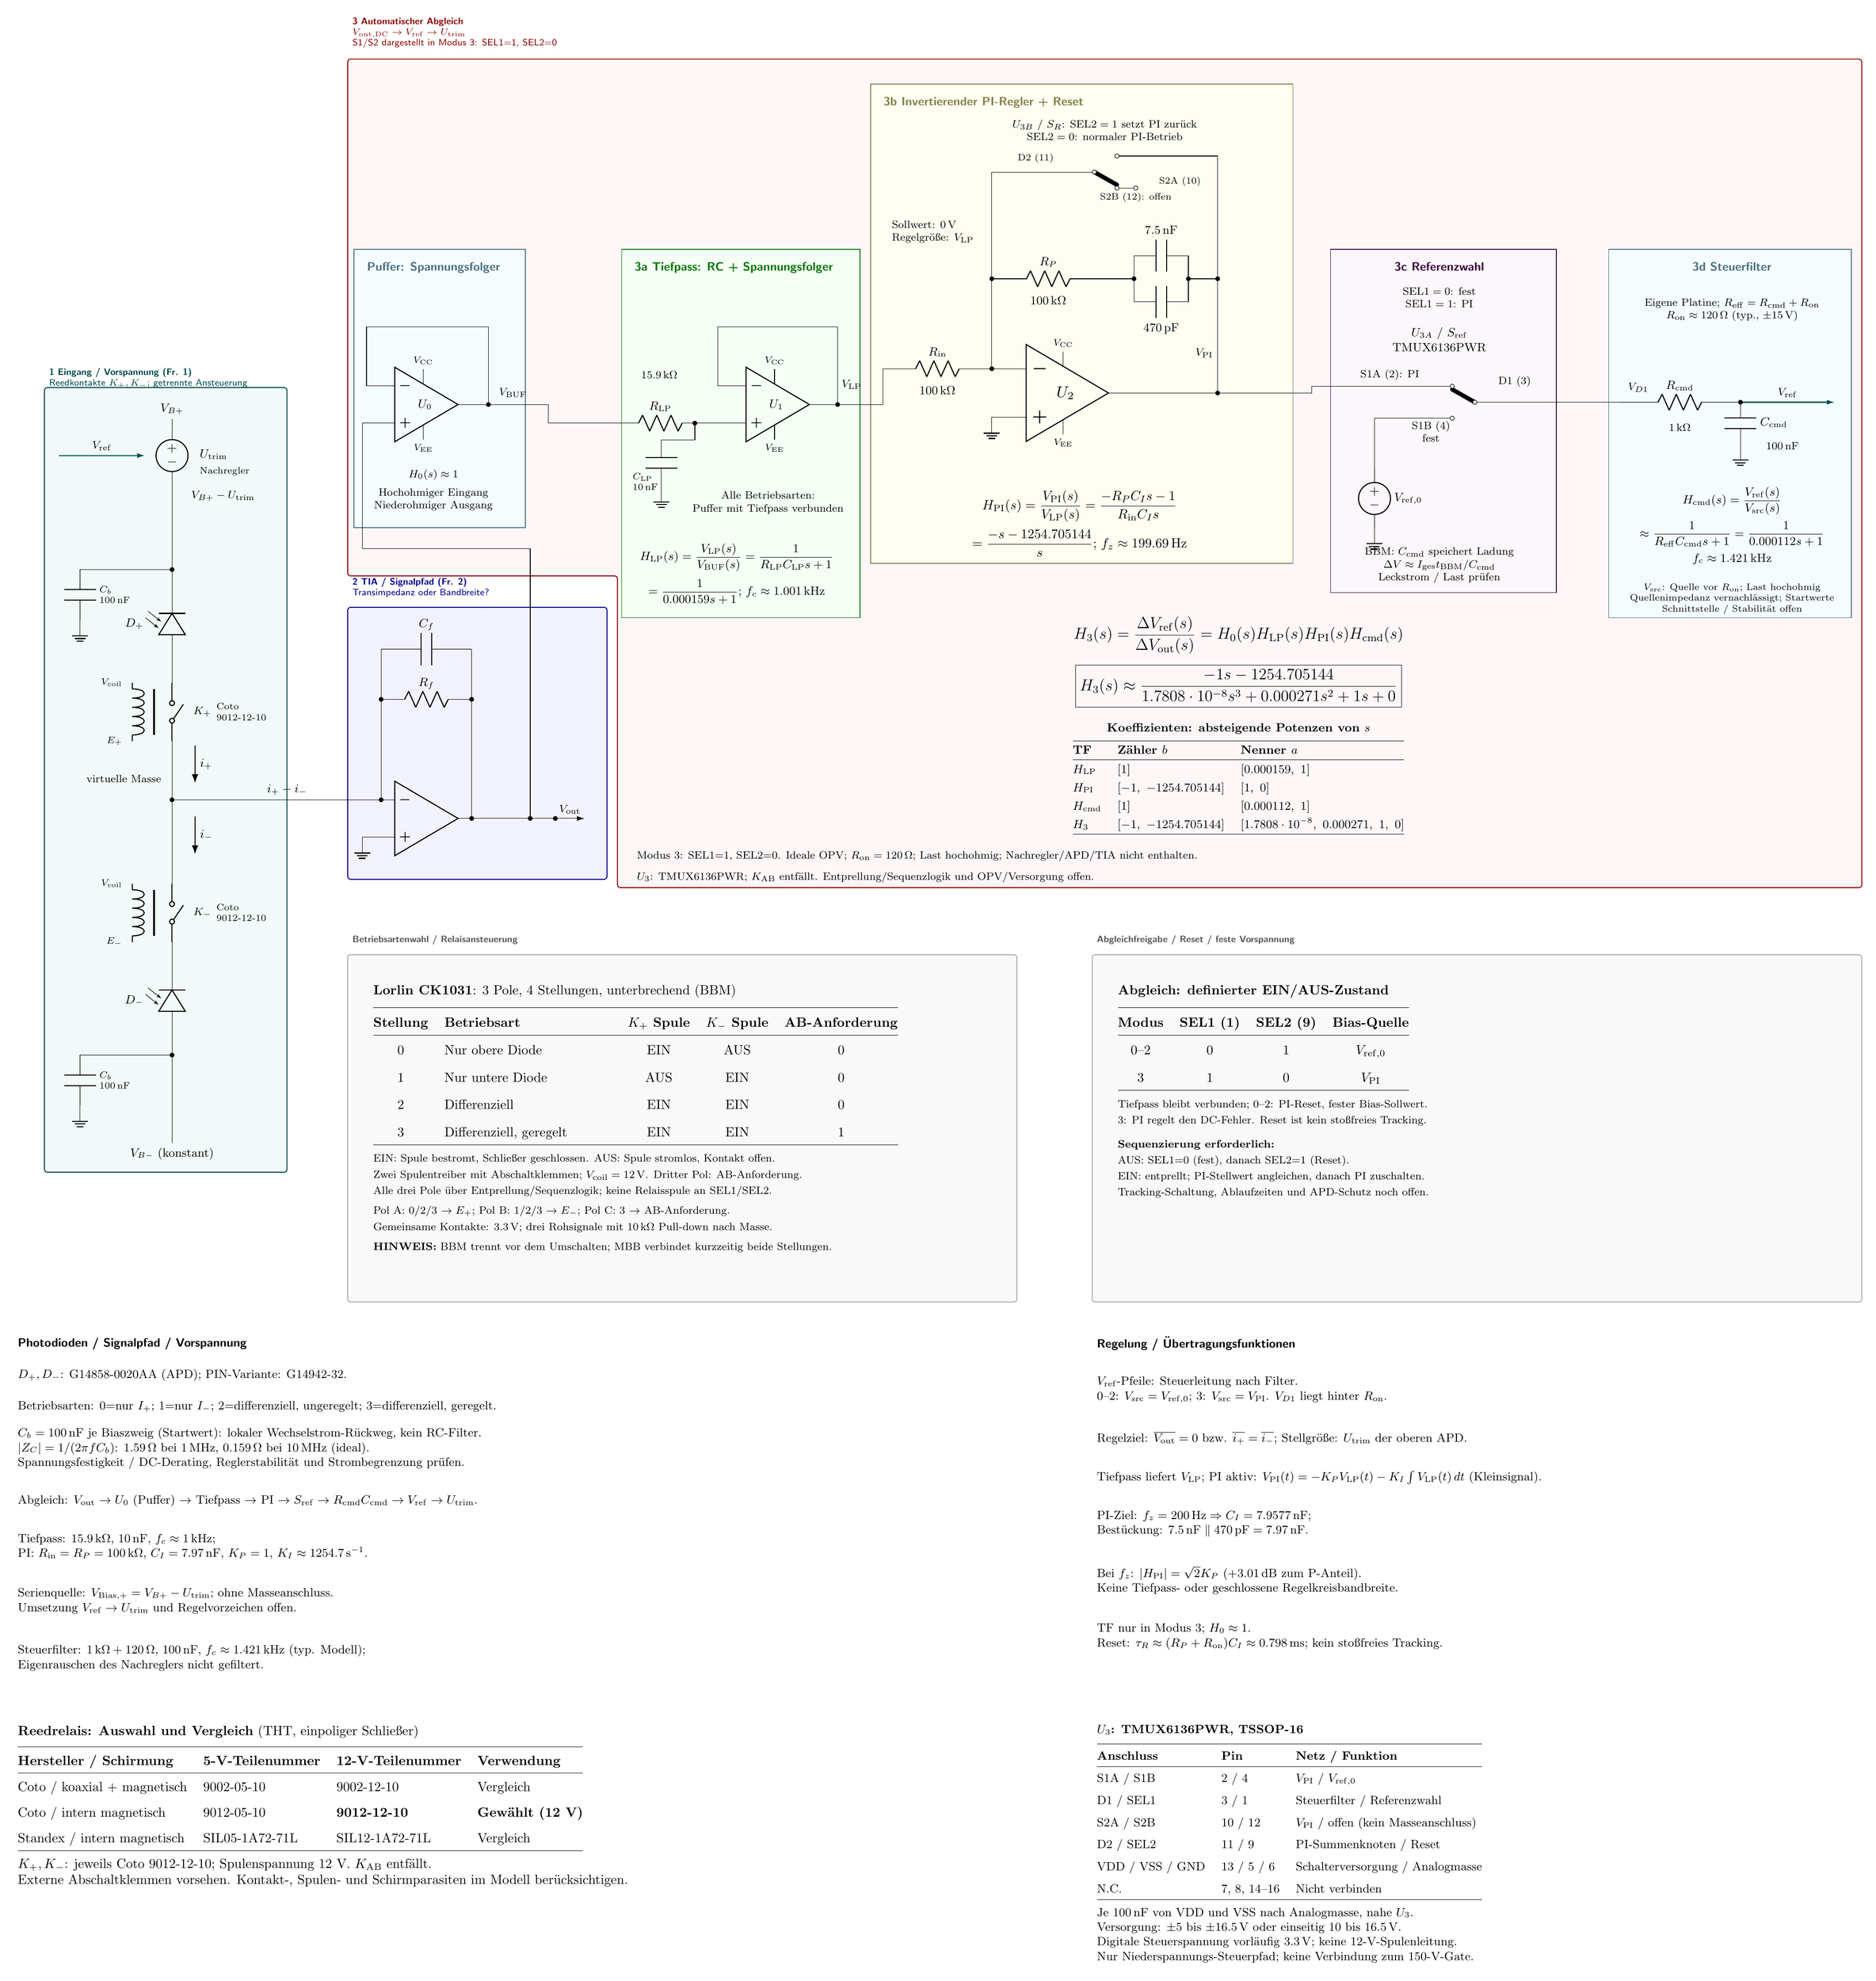
\begin{tikzpicture}[>=Latex, font=\small, x=1.1cm, y=1.1cm]
  \tikzset{control command/.style={
    draw=teal!65!black, line width=0.8pt,
    -{Latex[length=2mm,width=1.3mm]}}}

  %% ------------------------------------------------ reference coordinates
  \coordinate (bm)  at (0,-5.1);   % bias bypass tap, negative rail
  \coordinate (sum) at (0, 1.0);   % summing node = TIA virtual ground
  \coordinate (bp)  at (0, 6.5);   % bias bypass tap, positive rail

  %% ------------------------------------------------ floating series bias source
  \draw (0,10.1) node[above] {$V_{B+}$}
    to[american voltage source, name=trimsource]
    (0,8.35) coordinate (vbpreg);
  \node[anchor=west] at (0.55,9.25) {$U_{\rm trim}$};
  \node[anchor=west, font=\scriptsize] at (0.55,8.85) {Nachregler};
  \draw[control command] (-2.7,9.225) -- (-0.65,9.225)
    node[midway,above, font=\footnotesize] {$V_{\rm ref}$};

  %% ------------------------------------------------ main anti-series branch
  \draw (0,-7.2) node[below] {$V_{B-}$ (konstant)}
        -- (bm) -- (0,-4.8)
        to[pD, l=$D_-$] (0,-2.8)
        -- (0,-2.4);
  \draw (0,-1.0) -- (sum);
  \draw (sum) -- (0,2.4);
  \draw (0,3.8) -- (0,4.2)
        to[pD, l=$D_+$] (0,6.2)
        -- (bp) -- (vbpreg);
  \node[anchor=west, font=\footnotesize] at (0.35,8.25) {$V_{B+}-U_{\rm trim}$};

  %% ------------------------------------------------ reed relay symbols
  \foreach \yc/\suffix in {3.1/+,-1.7/-} {
    \pic at (0,\yc) {reed relay};
    \node[font=\scriptsize, anchor=east] at (-1.08,\yc+0.7) {$V_{\rm coil}$};
    \node[font=\scriptsize, anchor=east] at (-1.08,\yc-0.7) {$E_{\suffix}$};
    \node[font=\footnotesize, anchor=west] at (0.4,\yc) {$K_{\suffix}$};
    \node[font=\scriptsize, anchor=west, align=left] at (0.95,\yc)
      {Coto\\9012-12-10};
  }

  %% ------------------------------------------------ local bias bypass / AC ground
  \draw (bp) -- (-2.2, 6.5) to[C] (-2.2, 5.3) node[ground]{};
  \draw (bm) -- (-2.2,-5.1) to[C] (-2.2,-6.3) node[ground]{};
  \node[font=\scriptsize, anchor=west, align=left] at (-1.85,5.9)
    {$C_b$\\$100\,{\rm nF}$};
  \node[font=\scriptsize, anchor=west, align=left] at (-1.85,-5.7)
    {$C_b$\\$100\,{\rm nF}$};

  %% ------------------------------------------------ photocurrent direction
  \draw[-Latex, thick] (0.55, 2.30) -- (0.55, 1.40) node[midway,right] {$i_+$};
  \draw[-Latex, thick] (0.55, 0.60) -- (0.55,-0.30) node[midway,right] {$i_-$};
  \node[font=\footnotesize, anchor=east] at (-0.15,1.5) {virtuelle Masse};

  %% ------------------------------------------------ shared TIA
  \node[op amp, anchor=-] (oa) at (5.0,1) {};
  \draw (sum) -- node[pos=0.55, above] {$i_+ - i_-$} (oa.-);
  \draw (oa.+) -- ++(-0.45,0) node[ground]{};

  % feedback: R_f in parallel with C_f, both pinned to common y levels
  \coordinate (lvlR) at (0,3.4);
  \coordinate (lvlC) at (0,4.6);
  \draw (oa.-)   -- (oa.-   |- lvlR) coordinate (fa);
  \draw (oa.out) -- (oa.out |- lvlR) coordinate (fb);
  \draw (fa) to[R, l=$R_f$] (fb);
  \draw (fa) -- (fa |- lvlC) coordinate (ga);
  \draw (fb) -- (fb |- lvlC) coordinate (gb);
  \draw (ga) to[C, l=$C_f$] (gb);

  \draw (oa.out) -- ++(1.4,0) coordinate (abtap)
    -- ++(0.6,0) coordinate (vo);
  \draw[-{Latex[length=2mm,width=1.3mm]}] (vo) -- ++(0.7,0)
    node[pos=0.5,above, font=\footnotesize] {$V_{\rm out}$};

  %% ------------------------------------------------ TIA isolation follower
  \node[op amp, anchor=+] (bufamp) at (5.0,10.0) {$U_0$};
  \draw (abtap) -- (abtap |- 0,7.0) -- (4.55,7.0)
    -- (4.55,10.0) -- (bufamp.+);
  \draw (bufamp.out) -- ++(0.4,0) coordinate (bufout);
  \draw (bufamp.-) -- ++(-0.35,0) coordinate (bufminus)
    -- (bufminus |- 0,12.3) -- (bufout |- 0,12.3) -- (bufout);
  \draw (bufout) -- (9.0,0 |- bufout) -- (9.0,10.0) -- (10.85,10.0);
  \node[font=\footnotesize, anchor=south] at (8.15,10.5) {$V_{\rm BUF}$};
  \node[font=\footnotesize, align=center] at (6.25,8.4)
    {$H_0(s)\approx1$\\[4pt]
     Hochohmiger Eingang\\Niederohmiger Ausgang};

  %% ------------------------------------------------ LPF: RC + voltage follower
  \node[op amp, anchor=+] (lpfamp) at (13.4,10.0) {$U_1$};
  \draw (10.85,10.0) to[R, l=$R_{\rm LP}$]
    (12.5,10.0) coordinate (lpcap) -- (lpfamp.+);
  \node[font=\footnotesize, anchor=south] at (11.65,10.95) {$15.9\,{\rm k\Omega}$};
  \draw (lpcap) -- (12.5,9.6) -- (11.7,9.6) to[C]
    (11.7,8.5) node[ground]{};
  \node[font=\scriptsize, anchor=west, align=left] at (10.9,8.6)
    {$C_{\rm LP}$\\$10\,{\rm nF}$};
  \node[font=\footnotesize, align=center] at (14.25,8.1)
    {Alle Betriebsarten:\\Puffer mit Tiefpass verbunden};
  \draw (lpfamp.out) -- ++(0.35,0) coordinate (lpout);
  \draw (lpfamp.-) -- ++(-0.35,0) coordinate (lpminus)
    -- (lpminus |- 0,12.3) -- (lpout |- 0,12.3) -- (lpout);
  \draw (lpout) -- (16.55,0 |- lpout) coordinate (lpinter);
  \node[font=\footnotesize, anchor=south] at (16.25,10.7) {$V_{\rm LP}$};

  %% ------------------------------------------------ PI: series R-C feedback
  \node[op amp, scale=1.3, transform shape, anchor=-]
    (piamp) at (20.0,11.3) {$U_2$};
  \draw (lpinter) -- (17.0,0 |- lpinter) -- (17.0,11.3)
    to[R, l=$R_{\rm in}$] (19.6,11.3) coordinate (pisum) -- (piamp.-);
  \node[font=\small, anchor=north] at (18.3,11.0) {$100\,{\rm k\Omega}$};
  \draw (piamp.+) -- ++(-0.4,0) node[ground]{};
  \draw (piamp.out) -- (25.0,0 |- piamp.out) coordinate (piout);
  \draw (pisum) -- (19.6,13.45)
    to[R, l=$R_P$] (22.3,13.45) -- (23.0,13.45) coordinate (cileft);
  \draw (cileft) -- (23.0,14.0)
    to[C, l=$7.5\,{\rm nF}$] (24.3,14.0) -- (24.3,13.45) coordinate (ciright);
  \draw (cileft) -- (23.0,12.9)
    to[C, l_=$470\,{\rm pF}$] (24.3,12.9) -- (ciright);
  \draw (ciright) -- (25.0,13.45) -- (piout);
  \node[circ] at (19.6,13.45) {};
  \node[circ] at (25.0,13.45) {};
  \node[font=\small, anchor=north] at (20.95,13.15) {$100\,{\rm k\Omega}$};
  \coordinate (resetleft) at (19.6,16.0);
  \node[cute spdt down, anchor=in] (resetsel) at (22.0,16.0) {};
  \draw (pisum) -- (resetleft) -- (resetsel.in);
  \draw (resetsel.out 1) -- (25.0,0 |- resetsel.out 1) -- (piout);
  \draw (resetsel.out 2) -- ++(0.4,0) node[ocirc]{}
    node[below, font=\scriptsize] {S2B (12): offen};
  \node[font=\footnotesize, align=center] at (22.3,17.0)
    {$U_{3B}$ / $S_R$: $\mathrm{SEL2}=1$ setzt PI zur\"uck\\
     $\mathrm{SEL2}=0$: normaler PI-Betrieb};
  \node[font=\scriptsize, anchor=south] at (20.65,16.1) {D2 (11)};
  \node[font=\scriptsize, anchor=north] at (24.1,16.0) {S2A (10)};
  \node[font=\footnotesize, anchor=south east] at (25.0,11.45) {$V_{\rm PI}$};

  %% ------------------------------------------------ fixed/regulated reference selection
  \node[cute spdt up, xscale=-1, anchor=in] (refsel) at (31.2,10.5) {};
  \draw (piout) -- (27.25,0 |- piout)
    -- (27.25,0 |- refsel.out 1) -- (refsel.out 1);
  \coordinate (fixedref) at (28.75,8.9);
  \draw (fixedref) to[american voltage source, l=$V_{\rm ref,0}$]
    (28.75,7.5) node[ground]{};
  \draw (fixedref) -- (28.75,0 |- refsel.out 2) -- (refsel.out 2);
  \draw (refsel.in) -- (34.6,10.5) coordinate (cmdin);
  \node[font=\footnotesize, anchor=west] at (34.7,10.85) {$V_{D1}$};
  \node[font=\small, align=center] at (30.3,12.0)
    {$U_{3A}$ / $S_{\rm ref}$\\TMUX6136PWR};
  \node[font=\footnotesize, anchor=west] at (28.3,11.15) {S1A (2): PI};
  \node[font=\footnotesize, align=center] at (30.1,9.8) {S1B (4)\\fest};
  \node[font=\footnotesize, anchor=south] at (32.1,10.75) {D1 (3)};
  \node[font=\footnotesize, align=center] at (30.3,13.0)
    {$\mathrm{SEL1}=0$: fest\\$\mathrm{SEL1}=1$: PI};
  \node[font=\footnotesize, align=center] at (30.3,6.6)
    {BBM: $C_{\rm cmd}$ speichert Ladung\\
     $\Delta V\approx I_{\rm ges}t_{\rm BBM}/C_{\rm cmd}$\\
     Leckstrom / Last pr\"ufen};

  %% ------------------------------------------------ command filter on this board
  \begin{scope}[xshift=3.85cm]
  \draw (cmdin) to[R, l=$R_{\rm cmd}$] (34.0,10.5) coordinate (cmdout);
  \node[font=\footnotesize, anchor=north] at (32.55,10.1) {$1\,{\rm k\Omega}$};
  \draw (cmdout) to[C, l=$C_{\rm cmd}$] (34.0,9.5) node[ground]{};
  \node[font=\footnotesize, anchor=west] at (34.5,9.45) {$100\,{\rm nF}$};
  \draw[control command] (cmdout) -- (36.25,10.5)
    node[midway,above, font=\footnotesize] {$V_{\rm ref}$};
  \node[font=\footnotesize, align=center] at (33.8,12.7)
    {Eigene Platine; $R_{\rm eff}=R_{\rm cmd}+R_{\rm on}$\\
     $R_{\rm on}\approx120\,\Omega$ (typ., $\pm15\,{\rm V}$)};
  \node[font=\small, align=center] at (33.8,7.55)
    {$H_{\rm cmd}(s)=\dfrac{V_{\rm ref}(s)}{V_{\rm src}(s)}$
     \\[4pt]$\approx\dfrac{1}{R_{\rm eff}C_{\rm cmd}s+1}=\dfrac{1}{0.000112s+1}$
     \\[4pt]$f_c\approx1.421\,{\rm kHz}$};
  \node[font=\scriptsize, align=center] at (33.8,5.8)
    {$V_{\rm src}$: Quelle vor $R_{\rm on}$; Last hochohmig\\
     Quellenimpedanz vernachl\"assigt; Startwerte\\
     Schnittstelle / Stabilit\"at offen};
  \end{scope}

  \foreach \amp in {bufamp,lpfamp,piamp} {
    \draw (\amp.up) -- ++(0,0.35) node[above, font=\scriptsize] {$V_{\rm CC}$};
    \draw (\amp.down) -- ++(0,-0.35) node[below, font=\scriptsize] {$V_{\rm EE}$};
  }
  \foreach \junction in {bufout,lpcap,lpout,pisum,piout,cileft,ciright,cmdout}
    \node[circ] at (\junction) {};

  \node[align=center, font=\small] at (13.5,6.4)
    {$H_{\rm LP}(s)=\dfrac{V_{\rm LP}(s)}{V_{\rm BUF}(s)}=\dfrac{1}{R_{\rm LP}C_{\rm LP}s+1}$\\[5pt]
     $=\dfrac{1}{0.000159s+1}$; $f_c\approx1.001\,{\rm kHz}$};
  \node[align=center, font=\normalsize] at (21.7,7.6)
    {$H_{\rm PI}(s)=\dfrac{V_{\rm PI}(s)}{V_{\rm LP}(s)}
      =\dfrac{-R_PC_Is-1}{R_{\rm in}C_Is}$\\[5pt]
     $=\dfrac{-s-1254.705144}{s}$; $f_z\approx199.69\,{\rm Hz}$};
  \node[font=\footnotesize, anchor=west] at (11.0,-0.85)
    {$U_3$: TMUX6136PWR; $K_{\rm AB}$ entf\"allt. Entprellung/Sequenzlogik und OPV/Versorgung offen.};
  \node[align=center, font=\large] at (25.5,4.3)
    {$H_3(s)=\dfrac{\Delta V_{\rm ref}(s)}{\Delta V_{\rm out}(s)}
      =H_0(s)H_{\rm LP}(s)H_{\rm PI}(s)H_{\rm cmd}(s)$\\[7pt]
     $\boxed{H_3(s)\approx\dfrac{-1s-1254.705144}{1.7808\cdot10^{-8}s^3+0.000271s^2+1s+0}}$};
  \node[align=center, font=\small] at (25.5,1.5)
    {\textbf{Koeffizienten: absteigende Potenzen von $s$}\\[4pt]
     \renewcommand{\arraystretch}{1.25}%
     \begin{tabular}{@{}lll@{}}
       \hline
       \textbf{TF} & \textbf{Z\"ahler $b$} & \textbf{Nenner $a$}\\
       \hline
       $H_{\rm LP}$ & $[1]$ & $[0.000159,\ 1]$\\
       $H_{\rm PI}$ & $[-1,\ -1254.705144]$ & $[1,\ 0]$\\
       $H_{\rm cmd}$ & $[1]$ & $[0.000112,\ 1]$\\
       $H_3$ & $[-1,\ -1254.705144]$ & $[1.7808\cdot10^{-8},\ 0.000271,\ 1,\ 0]$\\
       \hline
     \end{tabular}};
  \node[font=\footnotesize, anchor=west] at (11.0,-0.35)
    {Modus 3: SEL1=1, SEL2=0. Ideale OPV; $R_{\rm on}=120\,\Omega$; Last hochohmig; Nachregler/APD/TIA nicht enthalten.};

  \foreach \junction in {bp,bm,sum,oa.-,fa,fb,oa.out,abtap,vo}
    \node[circ] at (\junction) {};

  %% ------------------------------------------------ mode control / coil drive
  \node[align=left, anchor=north west, font=\normalsize] at (4.7,-3.3)
    {\textbf{Lorlin CK1031}: 3 Pole, 4 Stellungen, unterbrechend (BBM)\\[6pt]
     \renewcommand{\arraystretch}{1.7}%
     \begin{tabular}{@{}cp{44mm}ccc@{}}
       \hline
       \textbf{Stellung} & \textbf{Betriebsart} & \textbf{$K_+$ Spule} & \textbf{$K_-$ Spule} & \textbf{AB-Anforderung}\\
       \hline
       0 & Nur obere Diode & EIN & AUS & 0\\
       1 & Nur untere Diode & AUS & EIN & 0\\
       2 & Differenziell & EIN & EIN & 0\\
       3 & Differenziell, geregelt & EIN & EIN & 1\\
       \hline
     \end{tabular}\\[6pt]
     {\footnotesize EIN: Spule bestromt, Schlie\ss er geschlossen. AUS: Spule stromlos, Kontakt offen.}\\
     {\footnotesize Zwei Spulentreiber mit Abschaltklemmen; $V_{\rm coil}=12\,{\rm V}$. Dritter Pol: AB-Anforderung.}\\
     {\footnotesize Alle drei Pole \"uber Entprellung/Sequenzlogik; keine Relaisspule an SEL1/SEL2.}\\[3pt]
     {\footnotesize Pol A: 0/2/3 $\rightarrow E_+$; Pol B: 1/2/3 $\rightarrow E_-$; Pol C: 3 $\rightarrow$ AB-Anforderung.}\\
     {\footnotesize Gemeinsame Kontakte: $3.3\,{\rm V}$; drei Rohsignale mit $10\,{\rm k\Omega}$ Pull-down nach Masse.}\\[3pt]
     {\footnotesize \textbf{HINWEIS:} BBM trennt vor dem Umschalten; MBB verbindet kurzzeitig beide Stellungen.}};

  \node[align=left, anchor=north west, font=\normalsize] at (22.5,-3.3)
    {\textbf{Abgleich: definierter EIN/AUS-Zustand}\\[6pt]
     \renewcommand{\arraystretch}{1.7}%
     \begin{tabular}{@{}cccc@{}}
       \hline
       \textbf{Modus} & \textbf{SEL1 (1)} & \textbf{SEL2 (9)} & \textbf{Bias-Quelle}\\
       \hline
       0--2 & 0 & 1 & $V_{\rm ref,0}$\\
       3 & 1 & 0 & $V_{\rm PI}$\\
       \hline
     \end{tabular}\\[6pt]
     {\footnotesize Tiefpass bleibt verbunden; 0--2: PI-Reset, fester Bias-Sollwert.}\\
     {\footnotesize 3: PI regelt den DC-Fehler. Reset ist kein sto\ss freies Tracking.}\\[6pt]
     {\footnotesize \textbf{Sequenzierung erforderlich:}}\\
     {\footnotesize AUS: SEL1=0 (fest), danach SEL2=1 (Reset).}\\
     {\footnotesize EIN: entprellt; PI-Stellwert angleichen, danach PI zuschalten.}\\
     {\footnotesize Tracking-Schaltung, Ablaufzeiten und APD-Schutz noch offen.}};

  %% ------------------------------------------------ caption
  \node[font=\sffamily\small, anchor=west] at (-3.8,-12.0)
    {\textbf{Photodioden / Signalpfad / Vorspannung}};
  \node[font=\sffamily\small, anchor=west] at (22.0,-12.0)
    {\textbf{Regelung / \"Ubertragungsfunktionen}};
  \node[font=\small, anchor=west] at (-3.8,-12.75)
    {$D_+,D_-$: G14858-0020AA (APD); PIN-Variante: G14942-32.};
  \node[font=\small, anchor=west] at (-3.8,-13.5)
    {Betriebsarten: 0=nur $I_+$; 1=nur $I_-$; 2=differenziell, ungeregelt; 3=differenziell, geregelt.};
  \node[font=\small, anchor=west, align=left] at (-3.8,-14.5)
    {$C_b=100\,{\rm nF}$ je Biaszweig (Startwert): lokaler Wechselstrom-R\"uckweg, kein RC-Filter.
     \\$|Z_C|=1/(2\pi f C_b)$: $1.59\,\Omega$ bei $1\,{\rm MHz}$, $0.159\,\Omega$ bei $10\,{\rm MHz}$ (ideal).
     \\Spannungsfestigkeit / DC-Derating, Reglerstabilit\"at und Strombegrenzung pr\"ufen.};
  \node[font=\small, anchor=west, align=left] at (-3.8,-15.75)
    {Abgleich: $V_{\rm out}\rightarrow U_0$ (Puffer) $\rightarrow$ Tiefpass $\rightarrow$ PI $\rightarrow S_{\rm ref}\rightarrow R_{\rm cmd}C_{\rm cmd}\rightarrow V_{\rm ref}\rightarrow U_{\rm trim}$.};
  \node[font=\small, anchor=west, align=left] at (-3.8,-16.85)
    {Tiefpass: $15.9\,{\rm k\Omega}$, $10\,{\rm nF}$, $f_c\approx1\,{\rm kHz}$;
     \\PI: $R_{\rm in}=R_P=100\,{\rm k\Omega}$, $C_I=7.97\,{\rm nF}$, $K_P=1$, $K_I\approx1254.7\,{\rm s}^{-1}$.};
  \node[font=\small, anchor=west, align=left] at (-3.8,-18.15)
    {Serienquelle: $V_{\rm Bias,+}=V_{B+}-U_{\rm trim}$; ohne Masseanschluss.
     \\Umsetzung $V_{\rm ref}\rightarrow U_{\rm trim}$ und Regelvorzeichen offen.};
  \node[font=\small, anchor=west, align=left] at (22.0,-13.1)
    {$V_{\rm ref}$-Pfeile: Steuerleitung nach Filter.
     \\0--2: $V_{\rm src}=V_{\rm ref,0}$; 3: $V_{\rm src}=V_{\rm PI}$. $V_{D1}$ liegt hinter $R_{\rm on}$.};
  \node[font=\small, anchor=west] at (22.0,-14.25)
    {Regelziel: $\overline{V_{\rm out}}=0$ bzw. $\overline{i_+}=\overline{i_-}$; Stellgr\"o\ss e: $U_{\rm trim}$ der oberen APD.};
  \node[font=\small, anchor=west] at (22.0,-15.2)
    {Tiefpass liefert $V_{\rm LP}$; PI aktiv: $V_{\rm PI}(t)=-K_PV_{\rm LP}(t)-K_I\int V_{\rm LP}(t)\,dt$ (Kleinsignal).};
  \node[font=\small, anchor=west, align=left] at (22.0,-16.3)
    {PI-Ziel: $f_z=200\,{\rm Hz}\Rightarrow C_I=7.9577\,{\rm nF}$;
     \\Best\"uckung: $7.5\,{\rm nF}\parallel470\,{\rm pF}=7.97\,{\rm nF}$.};
  \node[font=\small, anchor=west, align=left] at (22.0,-17.65)
    {Bei $f_z$: $|H_{\rm PI}|=\sqrt{2}K_P$ ($+3.01\,{\rm dB}$ zum P-Anteil).
     \\Keine Tiefpass- oder geschlossene Regelkreisbandbreite.};
  \node[font=\small, anchor=west, align=left] at (22.0,-19.0)
    {TF nur in Modus 3; $H_0\approx1$.
     \\Reset: $\tau_R\approx(R_P+R_{\rm on})C_I\approx0.798\,{\rm ms}$; kein sto\ss freies Tracking.};
  \node[font=\small, anchor=west, align=left] at (-3.8,-19.5)
    {Steuerfilter: $1\,{\rm k\Omega}+120\,\Omega$, $100\,{\rm nF}$, $f_c\approx1.421\,{\rm kHz}$ (typ. Modell);
     \\Eigenrauschen des Nachreglers nicht gefiltert.};
  \node[anchor=north west, font=\normalsize, align=left] at (-3.8,-21.0)
    {\textbf{Reedrelais: Auswahl und Vergleich} (THT, einpoliger Schlie\ss er)\\[5pt]
     \renewcommand{\arraystretch}{1.6}%
     \begin{tabular}{@{}llll@{}}
       \hline
       \textbf{Hersteller / Schirmung} & \textbf{5-V-Teilenummer} & \textbf{12-V-Teilenummer} & \textbf{Verwendung}\\
       \hline
       Coto / koaxial + magnetisch & 9002-05-10 & 9002-12-10 & Vergleich\\
       Coto / intern magnetisch & 9012-05-10 & \textbf{9012-12-10} & \textbf{Gew\"ahlt (12 V)}\\
       Standex / intern magnetisch & SIL05-1A72-71L & SIL12-1A72-71L & Vergleich\\
       \hline
     \end{tabular}\\[5pt]
     $K_+,K_-$: jeweils Coto 9012-12-10; Spulenspannung 12 V. $K_{\rm AB}$ entf\"allt.\\
     Externe Abschaltklemmen vorsehen. Kontakt-, Spulen- und Schirmparasiten im Modell ber\"ucksichtigen.};

  \node[anchor=north west, font=\small, align=left] at (22.0,-21.0)
    {\textbf{$U_3$: TMUX6136PWR, TSSOP-16}\\[5pt]
     \renewcommand{\arraystretch}{1.5}%
     \begin{tabular}{@{}lll@{}}
       \hline
       \textbf{Anschluss} & \textbf{Pin} & \textbf{Netz / Funktion}\\
       \hline
       S1A / S1B & 2 / 4 & $V_{\rm PI}$ / $V_{\rm ref,0}$\\
       D1 / SEL1 & 3 / 1 & Steuerfilter / Referenzwahl\\
       S2A / S2B & 10 / 12 & $V_{\rm PI}$ / offen (kein Masseanschluss)\\
       D2 / SEL2 & 11 / 9 & PI-Summenknoten / Reset\\
       VDD / VSS / GND & 13 / 5 / 6 & Schalterversorgung / Analogmasse\\
       N.C. & 7, 8, 14--16 & Nicht verbinden\\
       \hline
     \end{tabular}\\[5pt]
     Je $100\,{\rm nF}$ von VDD und VSS nach Analogmasse, nahe $U_3$.\\
     Versorgung: $\pm5$ bis $\pm16.5\,{\rm V}$ oder einseitig $10$ bis $16.5\,{\rm V}$.\\
     Digitale Steuerspannung vorl\"aufig $3.3\,{\rm V}$; keine 12-V-Spulenleitung.\\
     Nur Niederspannungs-Steuerpfad; keine Verbindung zum 150-V-Gate.};

  %% Functional regions; labels refer to the numbered tutor questions.
  \begin{scope}[on background layer]
    \draw[fill=teal!5, draw=teal!55!black, line width=0.7pt,
          rounded corners=2pt] (-3.05,-7.9) rectangle (2.75,10.85);
    \draw[fill=blue!5, draw=blue!55!black, line width=0.7pt,
          rounded corners=2pt] (4.2,-0.9) rectangle (10.4,5.6);
    \draw[fill=red!3, draw=red!55!black, line width=0.7pt,
          rounded corners=2pt] (4.2,6.35) -- (10.65,6.35) -- (10.65,-1.1)
          -- (40.4,-1.1) -- (40.4,18.7) -- (4.2,18.7) -- cycle;
    \draw[fill=cyan!4, draw=cyan!45!black, line width=0.6pt]
      (4.35,7.5) rectangle (8.45,14.15);
    \draw[fill=green!4, draw=green!45!black, line width=0.6pt]
      (10.75,5.35) rectangle (16.45,14.15);
    \draw[fill=yellow!5, draw=yellow!45!black, line width=0.6pt]
      (16.7,6.65) rectangle (26.8,18.1);
    \draw[fill=violet!3, draw=violet!45!black, line width=0.6pt]
      (27.7,5.95) rectangle (33.1,14.15);
    \draw[fill=cyan!4, draw=cyan!45!black, line width=0.6pt]
      (34.35,5.35) rectangle (40.15,14.15);
    \draw[fill=gray!5, draw=gray!65, line width=0.7pt,
          rounded corners=2pt] (4.2,-11.0) rectangle (20.2,-2.7);
    \draw[fill=gray!5, draw=gray!65, line width=0.7pt,
          rounded corners=2pt] (22.0,-11.0) rectangle (40.4,-2.7);
  \end{scope}
  \node[anchor=south west, align=left, font=\sffamily\scriptsize,
        text=teal!55!black] at (-3.05,10.72)
    {\textbf{1 Eingang / Vorspannung (Fr. 1)}\\
     Reedkontakte $K_+,K_-$; getrennte Ansteuerung};
  \node[anchor=south west, align=left, font=\sffamily\scriptsize,
        text=blue!55!black] at (4.2,5.72)
    {\textbf{2 TIA / Signalpfad (Fr. 2)}\\
     Transimpedanz oder Bandbreite?};
  \node[anchor=south west, align=left, font=\sffamily\scriptsize,
        text=red!55!black] at (4.2,18.85)
    {\textbf{3 Automatischer Abgleich}\\
     $V_{\rm out,DC} \rightarrow V_{\rm ref} \rightarrow U_{\rm trim}$\\
     S1/S2 dargestellt in Modus 3: SEL1=1, SEL2=0};
  \node[anchor=north west, font=\sffamily\small, text=green!45!black]
    at (10.95,13.95) {\textbf{3a Tiefpass: RC + Spannungsfolger}};
  \node[anchor=north west, font=\sffamily\small, text=yellow!45!black]
    at (16.9,17.9) {\textbf{3b Invertierender PI-Regler + Reset}};
  \node[anchor=north west, font=\sffamily\small, text=cyan!45!black]
    at (4.55,13.95) {\textbf{Puffer: Spannungsfolger}};
  \node[anchor=north, align=center, font=\sffamily\small, text=violet!45!black]
    at (30.3,13.95) {\textbf{3c Referenzwahl}};
  \node[anchor=north, align=center, font=\sffamily\small, text=cyan!45!black]
    at (37.3,13.95) {\textbf{3d Steuerfilter}};
  \node[anchor=north west, align=left, font=\footnotesize] at (17.1,14.95)
    {Sollwert: $0\,{\rm V}$\\Regelgr\"o\ss e: $V_{\rm LP}$};
  \node[anchor=south west, font=\sffamily\scriptsize, text=gray!65!black]
    at (4.2,-2.58) {\textbf{Betriebsartenwahl / Relaisansteuerung}};
  \node[anchor=south west, font=\sffamily\scriptsize, text=gray!65!black]
    at (22.0,-2.58) {\textbf{Abgleichfreigabe / Reset / feste Vorspannung}};

\end{tikzpicture}
\end{document}
